\section{Arranjos básicos e exemplos de circuitos}

\begin{frame}{Introdução aos arranjos}
\begin{block}{}
	Quando discutimos o exemplo do portão do sítio o acionamento do motor foi resolvido com um botão e um contator.
	\begin{itemize}
		\item Como fazemos para manter o portão aberto?
		\item Como fazemos para fechá-lo?
	\end{itemize}
	Os arranjos podem resolver esses problemas.
\end{block}

\centerline{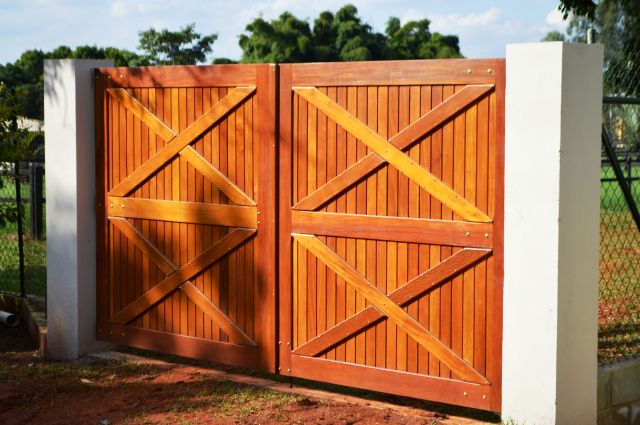
\includegraphics[width=0.6\linewidth]{Figuras/Ch07/fig0.jpg}}
\end{frame}

\begin{frame}{Exemplo \#01}
\begin{block}{Contextualização}
	Quando damos a partida em um carro, ele se mantém ligado até darmos outro comando (ou se deixarmos o motor ``morrer'').
	
	\begin{itemize}
		\item Como fazer o motor se ``lembrar'' da última ordem dada?
	\end{itemize}
\end{block}

\centerline{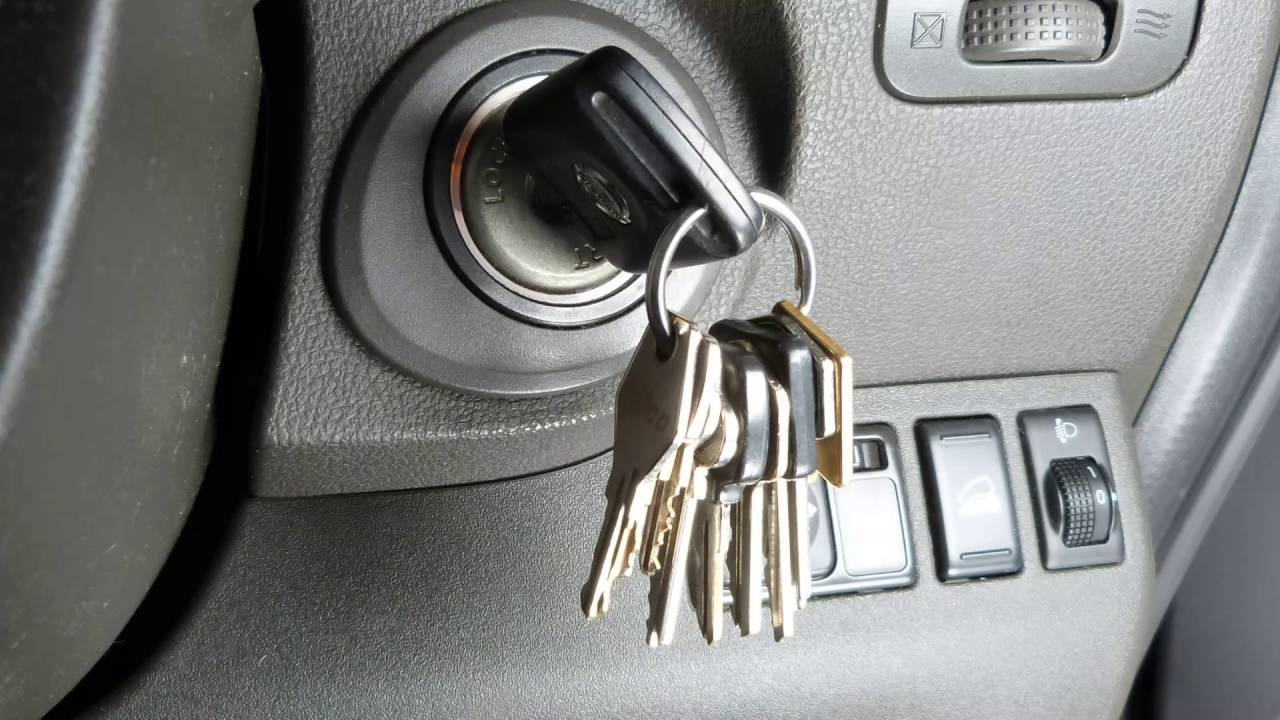
\includegraphics[width=0.8\linewidth]{Figuras/Ch07/fig1.jpg}}
\end{frame}


\begin{frame}{Exemplo \#01}
\begin{block}{Selo}
\begin{itemize}
    \item Podemos colocar uma chave auxiliar do contator do motor em paralelo com nosso botão de acionamento.
    \item Existe um problema com o circuito abaixo. Você consegue encontrá-lo?
\end{itemize}
\end{block}

\centerline{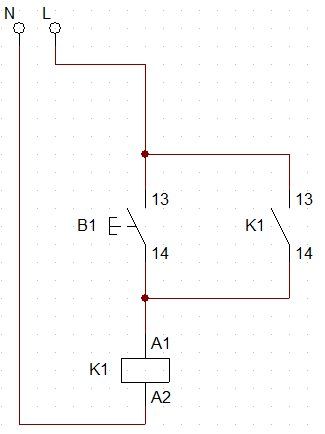
\includegraphics[height=0.65\textheight]{Figuras/Ch07/fig2.jpg}}
\end{frame}


\begin{frame}{Exemplo \#01}
\begin{block}{Selo}
\begin{itemize}
    \item O circuito de selo (ou de \textit{memória}) possui dois botões diferentes, um para ligá-lo e outro para desligá-lo.
\end{itemize}
\end{block}

\centerline{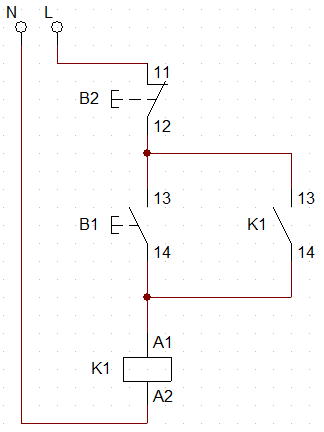
\includegraphics[height=0.7\textheight]{Figuras/Ch07/fig3.jpg}}
\end{frame}


\begin{frame}{Exemplo \#01}
\begin{block}{Selo}
\begin{itemize}
    \item Para \textbf{garantir} a memória em um circuito é possível colocar mais de um contator em paralelo com nossa chave de acionamento.
\end{itemize}
 \textbf{Nota:} A bobina de K2 não está representada.
\end{block}

\centerline{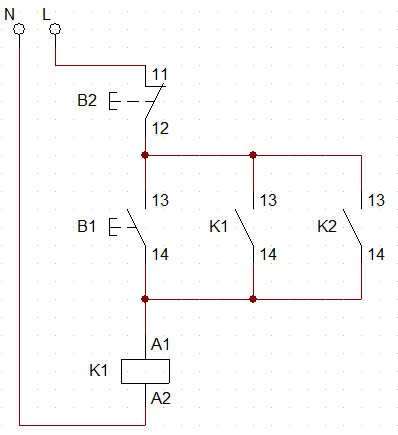
\includegraphics[height=0.55\textheight]{Figuras/Ch07/fig4.jpg}}
\end{frame}


\begin{frame}{Exemplo \#02}
\begin{block}{Contextualização}
\begin{itemize}
    \item Voltando ao nosso carro, precisamos dar ré para sair da garagem de casa.
    \item Como isso funciona?
\end{itemize}
\end{block}

\centerline{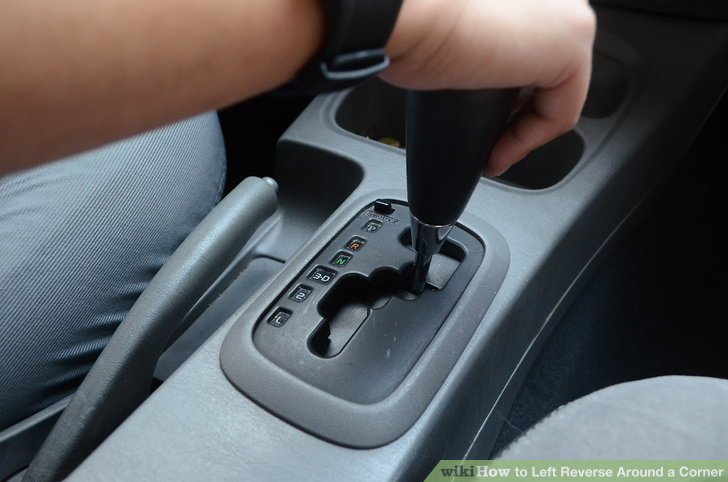
\includegraphics[width=0.65\linewidth]{Figuras/Ch07/fig5.jpg}}
\end{frame}


\begin{frame}{Exemplo \#02}
\begin{block}{Direção de rotação}
\begin{itemize}
    \item Em motores industriais podemos inverter a rotação de um motor invertendo duas de suas fases na entrada.
\end{itemize}
\end{block}
\begin{minipage}{0.45\linewidth}
	\centering
	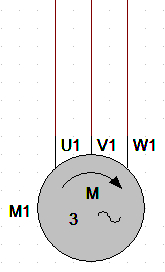
\includegraphics[width=0.6\linewidth]{Figuras/Ch07/fig6.jpg}
\end{minipage}
\hfill
\begin{minipage}{0.45\linewidth}
	\centering
	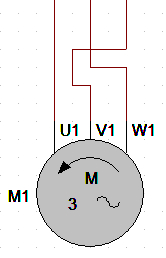
\includegraphics[width=0.65\linewidth]{Figuras/Ch07/fig7.jpg}
\end{minipage}
\end{frame}


\begin{frame}{Exemplo \#02}
\begin{block}{Direção de rotação}
\begin{itemize}
    \item Se quisermos fazer nosso motor mudar de rotação com o apertar de um botão (ou engatando uma marcha específica) podemos fazer um circuito com dois contatores, cada um em uma configuração de rotação específica.
\end{itemize}
\end{block}
\centerline{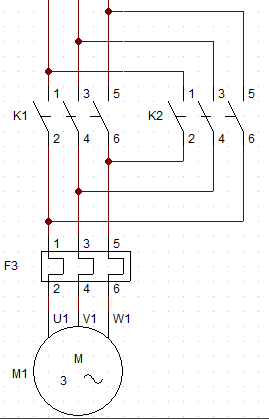
\includegraphics[height=0.6\textheight]{Figuras/Ch07/fig8.jpg}}
\end{frame}


\begin{frame}{Exemplo \#02}
\begin{block}{Intertravamento}
\begin{itemize}
    \item Se ligarmos esses dois contatores ao mesmo tempo fecharemos um curto em nosso motor.
    \item Para resolver esse problema usamos o \textbf{intertravamento}.
\end{itemize}
\end{block}
\centerline{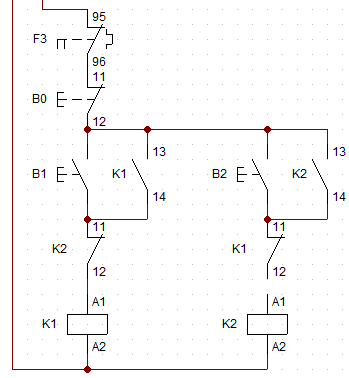
\includegraphics[height=0.6\textheight]{Figuras/Ch07/fig9.jpg}}
\end{frame}

\begin{frame}{Exemplo \#02}
\begin{block}{Intertravamento}
\begin{itemize}
    \item Quando apertamos o botão B1, o contator K1 se aciona e abre a passagem que liga o contator K2. O mesmo acontece se apertarmos B2 e K1 estiver em repouso.
    \item Um contator ``trava'' o funcionamento do outro.
    \item É \textbf{essencial} que a chave auxiliar que realiza a trava esteja em \textbf{série} com o circuito de acionamento do contator que deve travar, caso contrário a trava não funciona.
\end{itemize}
\end{block}
\end{frame}


\begin{frame}{Exemplo \#02}
\begin{block}{Intertravamento}
\begin{itemize}
    \item Se quisermos aumentar o nível de segurança podemos compor a trava com mais chaves auxiliares.
\end{itemize}
\end{block}
\centerline{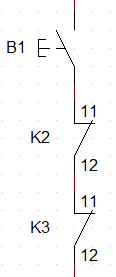
\includegraphics[width=0.2\linewidth]{Figuras/Ch07/fig10.jpg}}
\end{frame}


\begin{frame}{Exemplo \#02}
\begin{block}{Ligamento condicional}
\begin{itemize}
    \item Uma configuração com o efeito oposto ao do intertravamento é o \textit{ligamento condicional}.
\end{itemize}
\end{block}
\centerline{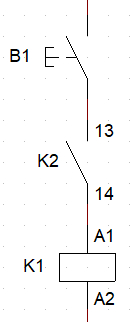
\includegraphics[width=0.2\linewidth]{Figuras/Ch07/fig11.jpg}}
\end{frame}


\begin{frame}{Exemplos de circuitos elétricos}
\begin{block}{}
	Agora, vamos ilustrar alguns circuitos utilizados comumente para acionar motores.
	
	Os elementos básicos nos comandos elétricos são:
	
	\begin{itemize}
		\item Dispositivos de manobra
		\item Dispositivos de proteção (curto e sobrecarga)
		\item Seccionamento
		\item Equipamento de potência
	\end{itemize}

	Você consegue identificar esses elementos nos exemplos?
\end{block}
\end{frame}


\begin{frame}{Partida direta}
\centerline{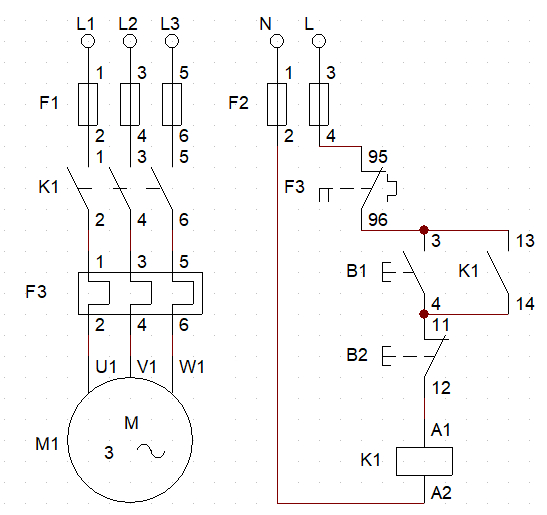
\includegraphics[width=0.7\linewidth]{Figuras/Ch07/fig12.jpg}}
\end{frame}

\begin{frame}{Partida direta com sinalização}
\centerline{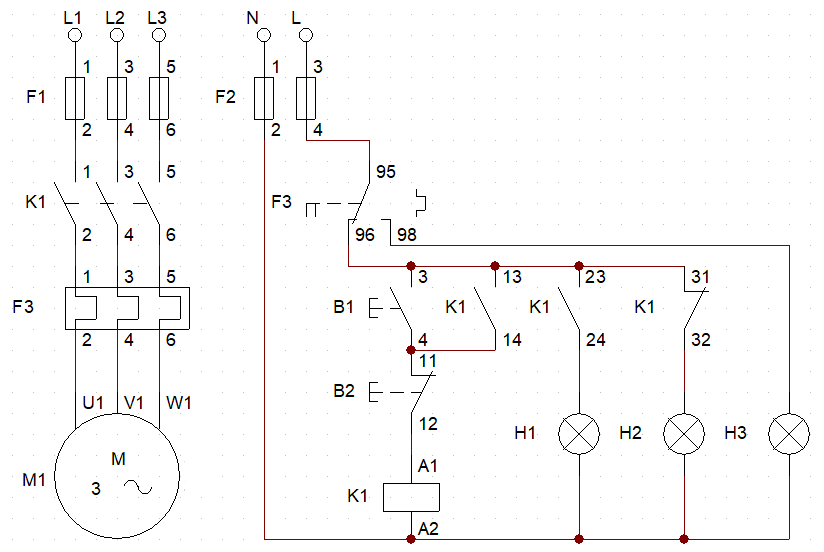
\includegraphics[width=1\linewidth]{Figuras/Ch07/fig13.jpg}}
\end{frame}

\begin{frame}{Partida direta com reversão}
\centerline{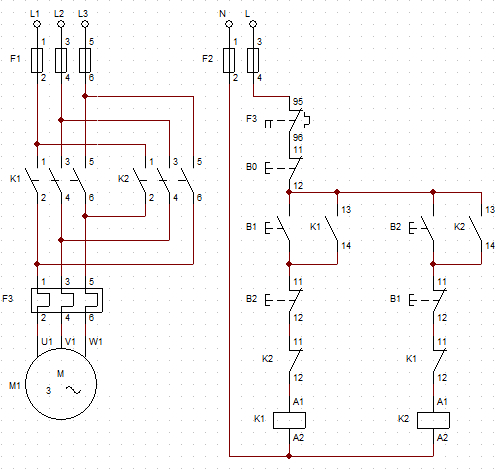
\includegraphics[height=0.9\textheight]{Figuras/Ch07/fig14.jpg}}
\end{frame}


\begin{frame}{Exemplos de circuitos elétricos}
\begin{block}{Tipos de partidas}
\begin{itemize}
    \item Motores industriais são equipamentos caros e que precisam de cuidados especiais.
    \item Existem diferentes formas acionar um motor, cada qual com seus benefícios e fraquezas.
    \item Vamos explorar três formas de acionar um motor usando ligações estrela e triângulo.
\end{itemize}
\end{block}
\end{frame}


\begin{frame}{Exemplos de circuitos elétricos}
\begin{block}{Princípio das ligações de motores}
\begin{itemize}
    \item Um motor trifásico é composto por três bobinas que podem ser ligadas entre si de diferentes maneiras.
\end{itemize}
\end{block}
\centerline{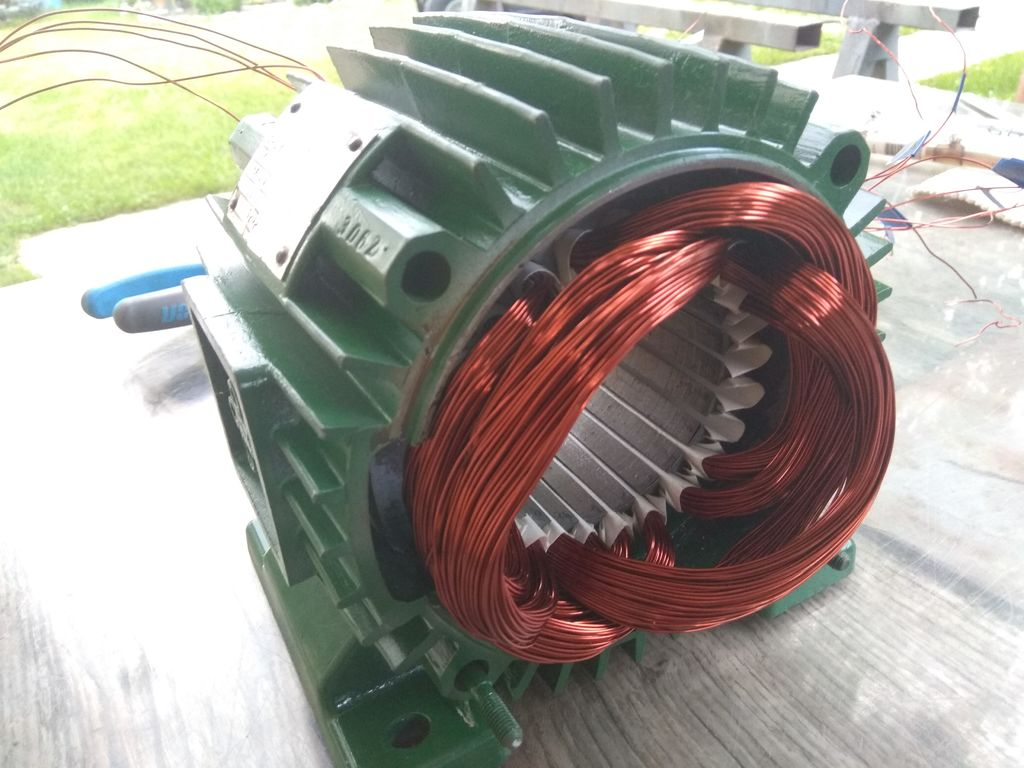
\includegraphics[width=0.6\linewidth]{Figuras/Ch07/fig15.jpg}}
\end{frame}


\begin{frame}{Exemplos de circuitos elétricos}
\begin{block}{Princípio das ligações de motores}
\begin{itemize}
    \item Em eletrônica podemos conectar três bobinas das seguintes maneiras:
\end{itemize}
\end{block}

\vspace{1.5cm}
\begin{minipage}{0.45\linewidth}
	\centering
	\begin{circuitikz}[x=1.5cm, y=1.5cm]
		\draw (0,1) to[short, o-*] ++(1,0) to[L] ++(0,-1) to[short, *-o] ++(-1,0);
		\draw (1,1) to[short, -*] ++(1,0) to[L] ++(0,-1) to[short, *-] ++(-1,0);
		\draw (2,1) to[short] ++(1,0) to[L] ++(0,-1) to[short] ++(-1,0);
	\end{circuitikz}
	
	Em paralelo
\end{minipage}
\hfill
\begin{minipage}{0.45\linewidth}
	\centering
	\begin{circuitikz}[x=1.5cm, y=1.5cm]
		\draw (0,1) to[short, o-] ++(0.2,0) to[L] ++(1,0) to[L] ++(1,0) to[L] ++(1,0) to[short, -o] ++(0.2,0);
	\end{circuitikz}
	
	Em série
\end{minipage}
\end{frame}


\begin{frame}{Exemplos de circuitos elétricos}
\begin{block}{Princípio das ligações de motores}
	Mas, como estamos lidando com um sistema trifásico, precisamos adaptar um pouco.
\end{block}

\vspace{0.5cm}
\begin{minipage}{0.45\linewidth}
	\centering
	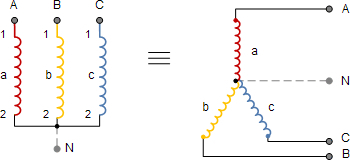
\includegraphics[width=\linewidth]{Figuras/Ch07/fig16.jpg}
	
	Em paralelo, o que vamos chamar de \textbf{estrela} (Y)
\end{minipage}
\hfill
\begin{minipage}{0.45\linewidth}
	\centering
	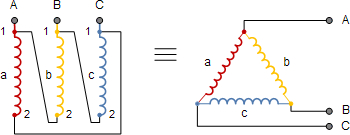
\includegraphics[width=\linewidth]{Figuras/Ch07/fig17.jpg}
	
	Em série, o que vamos chamar de \textbf{triângulo} ($ \Delta $)
\end{minipage}

\end{frame}

\begin{frame}{Exemplos de circuitos elétricos}
\begin{block}{Ligação Y}
\begin{itemize}
    \item Na ligação estrela nosso motor tem menos força, e por isso, se estiver parado, sentirá menos impacto quando for acionado.
    \item É ideal para \textbf{ligar} o motor, mas \textbf{não} para \textbf{trabalhar} com ele.
\end{itemize}
\end{block}
\end{frame}


\begin{frame}{Exemplos de circuitos elétricos}
\centerline{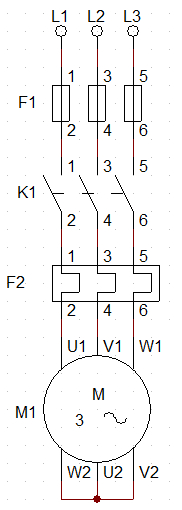
\includegraphics[height=0.9\textheight]{Figuras/Ch07/fig18.jpg}}
\end{frame}


\begin{frame}{Exemplos de circuitos elétricos}
\begin{block}{Ligação $ \Delta $}
\begin{itemize}
    \item Na ligação triângulo nosso motor tem mais força, por isso é usada na hora de trabalhar com grandes cargas.
    \item É ideal para \textbf{trabalhar} com motor, mas \textbf{não} para \textbf{acioná-lo}.
\end{itemize}
\end{block}
\end{frame}


\begin{frame}{Exemplos de circuitos elétricos}
\centerline{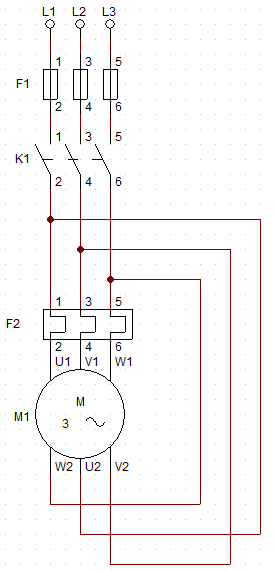
\includegraphics[height=0.9\textheight]{Figuras/Ch07/fig19.jpg}}
\end{frame}


\begin{frame}{Exemplos de circuitos elétricos}
\begin{block}{Partida Y-$ \Delta $}
\begin{itemize}
    \item Podemos unir o útil ao agradável através do uso de \textbf{temporizadores}, dando a partida no nosso motor usando a ligação estrela e, depois, trabalhar com ele na ligação triângulo.
\end{itemize}
\end{block}
\end{frame}


\begin{frame}{Exemplos de circuitos elétricos}
\centerline{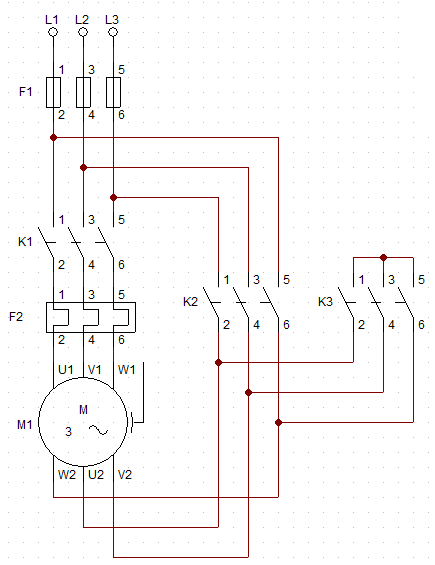
\includegraphics[height=0.9\textheight]{Figuras/Ch07/fig20.jpg}}
\end{frame}


\begin{frame}{Exemplos de circuitos elétricos}
\centerline{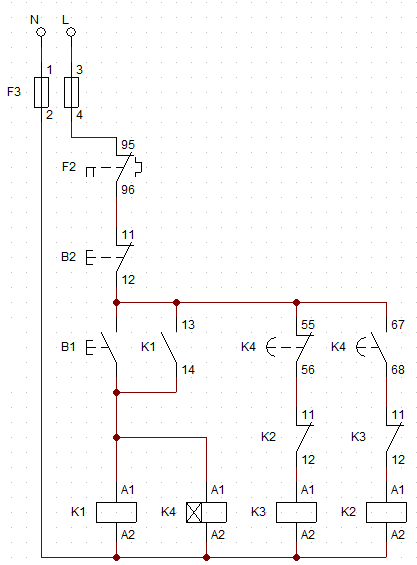
\includegraphics[height=0.9\textheight]{Figuras/Ch07/fig21.jpg}}
\end{frame}


\begin{frame}{Exemplos de circuitos elétricos}
\centerline{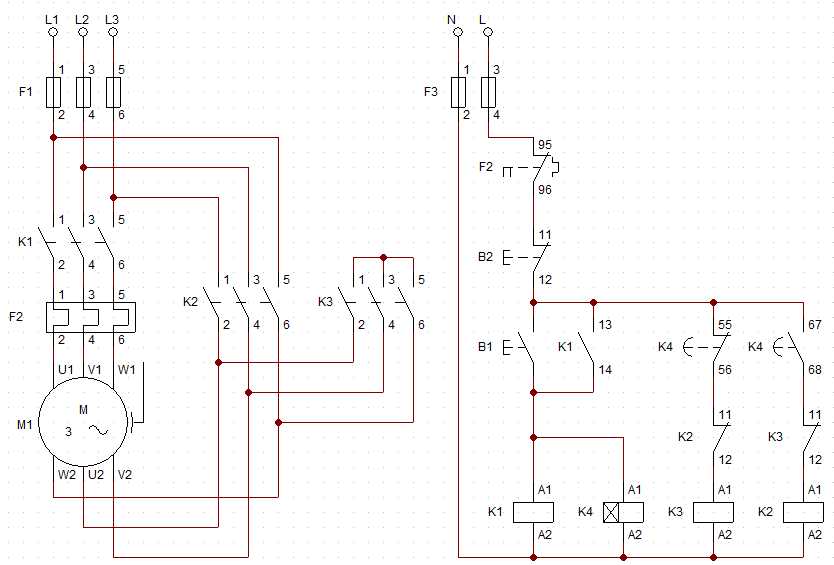
\includegraphics[height=0.9\textheight]{Figuras/Ch07/fig22.jpg}}
\end{frame}


\frame{
	\frametitle{Exercícios}
	\begin{block}{}
		01. Dar um exemplo de uso de dois arranjos em conjunto.
		
		\vspace{0.5cm}
		
		02. Esboçar o circuito do exemplo dado na questão 01.
	\end{block}
}

\section*{Referências}
\frame{
	\frametitle{Referências e Exercícios Complementares}
	\begin{itemize}
		\item FILHO, João Mamede. Instalações Elétricas Industriais, 6 ed. Rio de Janeiro, LTC, 2001.
	\end{itemize}
	%\centering{\alert{Página 546 - \textbf{Capítulo 6}}} \\
	%\centering{\alert{Lista de exercícios 01}}
}